\chapter{Visceral Leishmaniasis}
\label{applications-priors_empirical}

Moving away from more `subjective' expert priors, empirical priors rely on the data.  Similar to fitting the complete hierarchical model, empirical priors use predictions from a simple global model to inform parallel regional models, as discussed in Chapter \ref{theory-age_pattern_model}.  In modeling diseases with insufficient data for all geographic areas, such as visceral leishmaniasis (VL), empirical priors provide data-derived relationships to guide the modeling process.

Visceral leishmaniasis is a parasitic disease in which the parasite invades cells in the liver, spleen, bone marrow and lymph nodes.  If untreated, it causes life-threatening systemic infection.  Diagnosis includes identification of the parasite in tissue samples, ideally from the spleen or bone marrow.  The parasite is transmitted by several species of sandflies.  Traditionally  endemic in the tropics, subtropics and southern Europe, VL is becoming a common AIDS-associated opportunistic infection \cite{herwaldt_leishmaniasis_1999, zeledon_hemoflagellates_1996}.

Data is primarily from hospital admissions data, but also includes data from systematic review.  Only population representative data were included for the analysis, specific population groups and cases of HIV-coinfection were excluded.  Thus the analysis includes 3583 rows of data from 12 regions.

    \begin{figure}[h]
        \begin{center}
            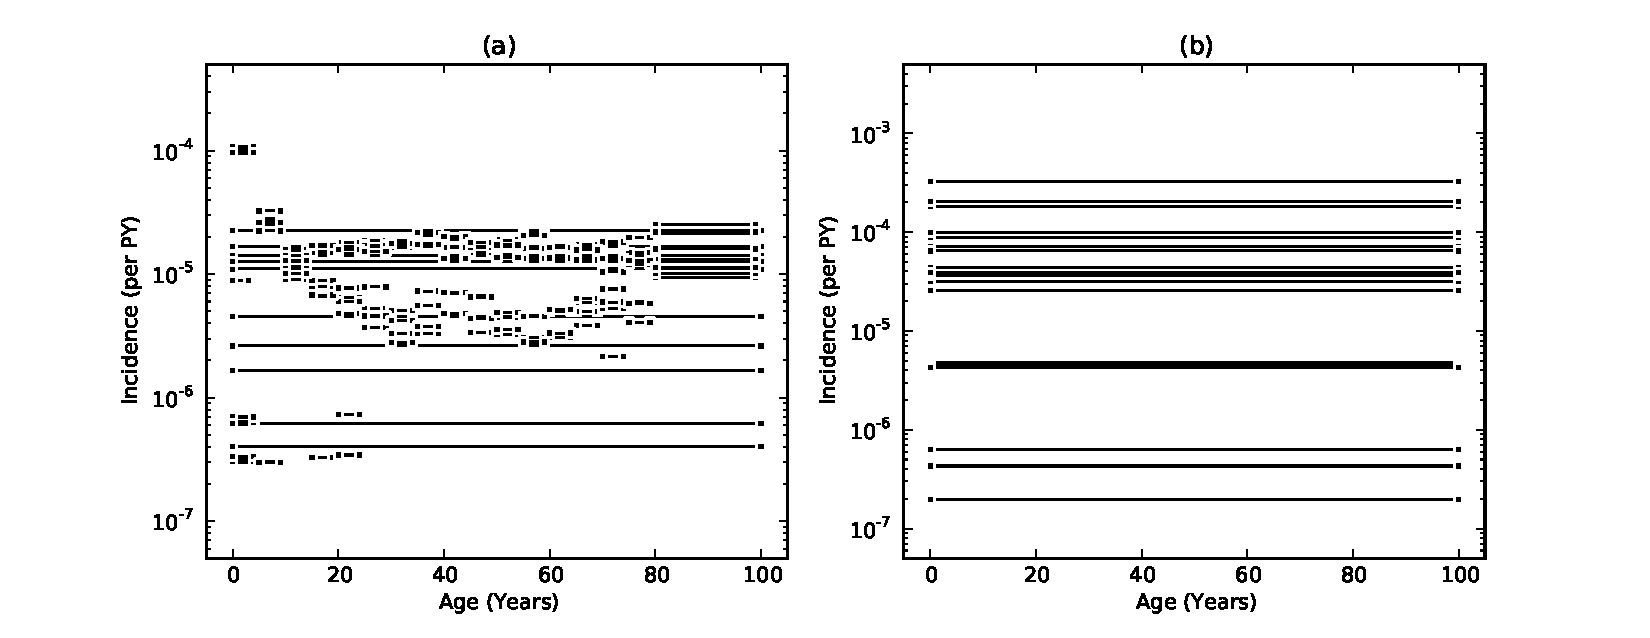
\includegraphics[width=\textwidth]{vl-data.pdf}
            \caption{Visceral leishmaniasis incidence data from systematic review for super-region 6 (a) and super-region 2 (b).}
            \label{fig:app-vl data}
        \end{center}
    \end{figure}

Super-region 6, composed of the Caribbean, central, Andean and tropical Latin America, has low incidence.  However it has an age-pattern that can be used as an empirical prior for areas without an age-pattern, such as super-region 2 (sub-Saharan Africa).  Figure \ref{fig:app-vl data} shows the available data for these super-regions.  Unless there is data to inform otherwise, the highest hierarchal level assumes the empirical prior is true.



\ref{fig:app-vl pred compare}

    \begin{figure}[h]
        \begin{center}
            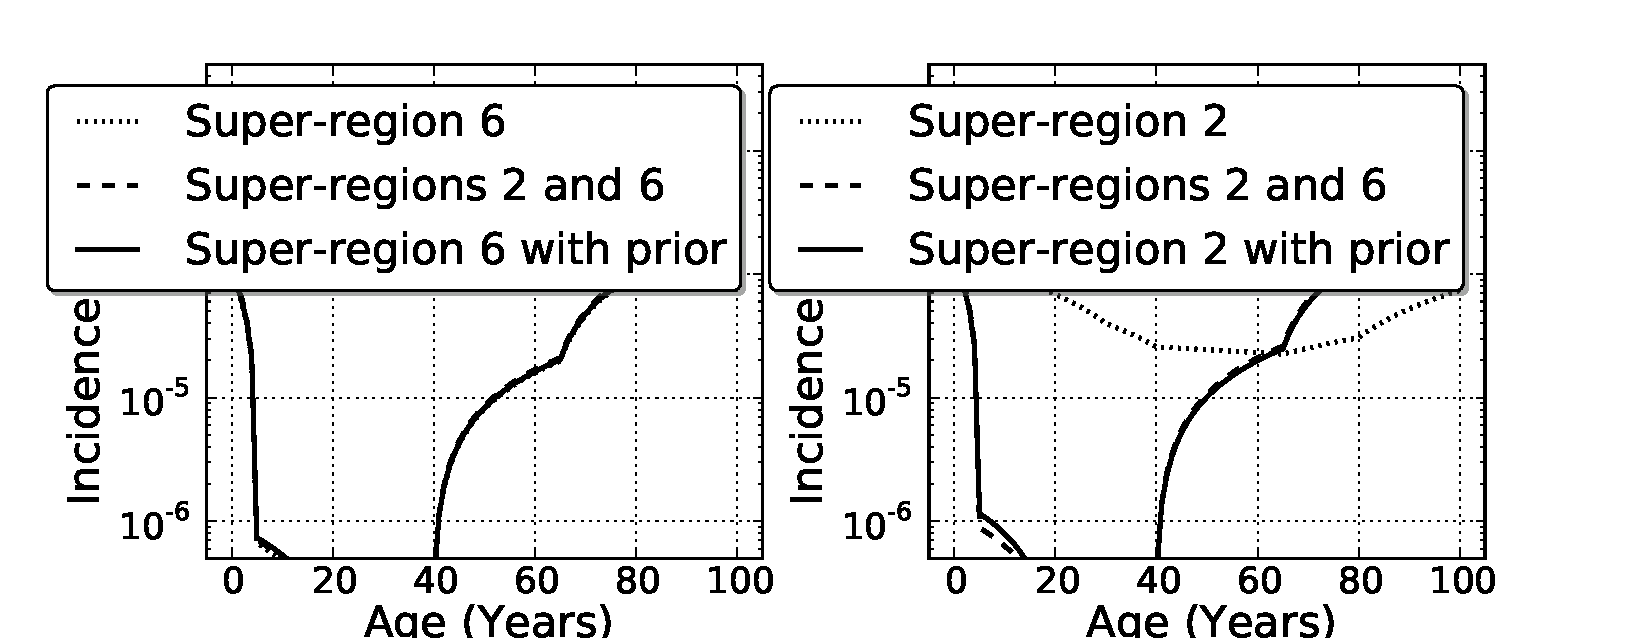
\includegraphics[width=\textwidth]{vl-pred_compare.pdf}
            \caption{.}
            \label{fig:app-vl pred compare}
        \end{center}
    \end{figure} 